\section{Introduction}
Many applications receive input data as files. These files must usually adhere to a specific format in order
to be accepted by the application since it is common practice to swiftly discard inputs should they not pass a
conformity check. Examples of such checks include schema validation and checksum verification. Typically, these
checks are of no interest when testing such applications as the goal is rather testing the logic of the
application itself; however, they present an obstacle when generating inputs for
testing purposes.

Creating test inputs in sufficient quantities manually is often infeasible because of the overwhelming number
of values that need to be produced -- possibly in different combinations and successions -- which is why in
these cases automatic testing is the only viable alternative. Several ideas can be explored to enable automatic
testing techniques to produce test inputs which pass conformity checks and improve the quality of the
resulting tests as much as possible.

The first idea is to leverage the same format definitions that are used for the checks when generating the
inputs. For an example consider an \xsd, which describes the format of a concrete \xml dialect, it contains all
the information necessary to generate instances of this dialect. Another example is the \png file format
documentation, which describes all values that are legal in \png files.

The second idea is to occasionally ignore some parts of the specification with the goal of producing inputs
that reveal vulnerabilities in the application under test. This is especially important as all such exposures
present a real threat to security or usability because tests of real usage scenarios (i.e.\ system level tests)
cannot produce false positives by definition.

The third idea is to benefit from search-based techniques when generating test inputs in order to increase
effectiveness by steering the production of inputs towards desired properties or particular testing goals.
Examples of such goals include specific classes of security vulnerabilities like integer or buffer overflows.

\xmlmate{}\cite{Havrikov:2014:XEX:2635868.2661666} is a tool that already implements most of these ideas to
some extent -- it is capable of generating \xml instances from an \xsd{}, and optionally additional \xml
samples, using a search-based genetic algorithm based on \evosuite{}\cite{fraser2013whole}. \xmlmate is
primarily aimed at \java applications that process \xml files, however, it is very well-suited to be extended
to work with non-\java programs, non-\xml formats, and vulnerability-oriented guidance criteria for its
search-based input generation algorithm.

The goal of this thesis is to provide \xmlmate with prototypical implementations of these extensions and
evaluate their effectiveness and efficiency on several real-world test subjects, and thus determine the
viability of the proposed ideas for enhancing test input generation techniques in the context of automated system testing.

\Cref{fig:overview} shows a schematic overview of the proposed extended \xmlmate process.
% non-xml
The core component of \xmlmate produces \xml files according an \xsd. 
The files are transformed by means of a converter component if the program under test expects a different
format. This removes \textsc{XMLMate's} limitation of being able to produce only \xml-based inputs.
% non-java
While the program under test is executed with the converted files as inputs, a fitness function component
injected into it gathers data on the inputs' effects.
% vulnoriented fitfuncs
There are several fitness functions, each calibrated to different effects e.g.\ specific security vulnerability
symptoms. 
Upon receiving the data from the fitness function component, the \xmlmate core ranks the current inputs,
selects the best and evolves them by changing them according to specific rules, while occasionally introducing
values that violate the specification in the governing \xsd. 
These modified input files make up the next generation, to be converted and fed into the program under test as
before. 
In this manner inputs are improved iteratively towards inducing desired behavior in the program under test. 

\begin{figure}[htb]
\centering
  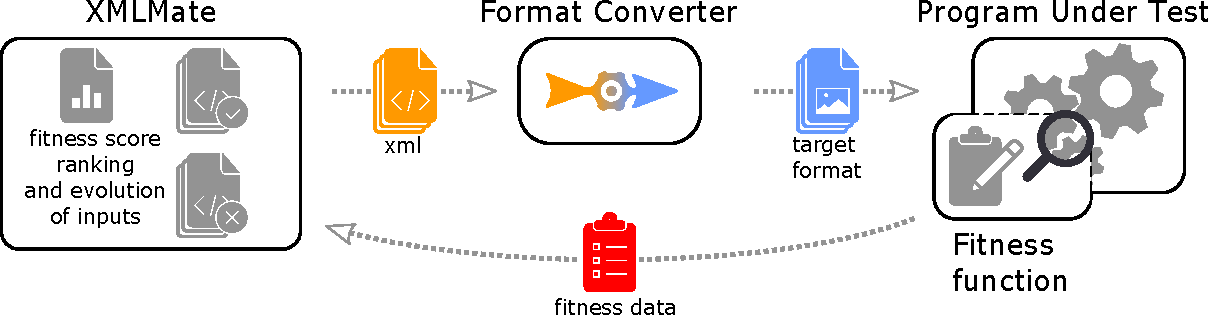
\includegraphics[width=\columnwidth]{overview.pdf}
  \caption{Schematic Overview of \xmlmate's Extended Process}
  \label{fig:overview}
\end{figure}

The remainder of this document is organized as follows: \cref{sec:relwork} gives an overview of approaches
related to the one proposed, which is itself described in great detail in \cref{sec:approach}, including the
technology stack used, the components the system consists of, challenges encountered during implementation and
their solutions, as well as guidance function and file format descriptions. The evaluation setup and
experimental results are presented in \cref{sec:evaluation}, whereafter \cref{sec:conclusion} provides a
conclusion statement, followed by an outlook on future enhancements and challenges.
